\documentclass[14px]{article}
\usepackage{xeCJK}
\usepackage[frenchb]{babel}
\usepackage[T1]{fontenc}
\usepackage[utf8]{inputenc}
\usepackage{textcomp}
\usepackage{amssymb}
\usepackage[ruled,longend]{algorithm2e}
\usepackage{amsmath}
\usepackage{latexsym}
\usepackage{fancyhdr}
\usepackage{geometry}
\usepackage{setspace}
\usepackage[colorlinks,linkcolor=blue]{hyperref}
% Image
\usepackage{graphicx}
\usepackage{float}
\usepackage{subfigure}
\usepackage{enumerate}

\begin{document}
\setlength{\parindent}{0pt}
\begin{titlepage}
	\begin{center}
		% Upper part of the page
		
\includegraphics[width=0.35\textwidth]{logo.png}\\[1cm]
		\textsc{\Large Rapport de PC3R}\\[0.5cm]
		% Title
		{ \huge \bfseries Système de Gestion de Location}\\[0.4cm]
		% Author and supervisor
		\begin{minipage}{0.4\textwidth}
			\begin{flushleft} \large
				\emph{Author:}\\
				Qiwei \textsc{XIAN}\\
				Ruiwen \textsc{WANG}\\
			\end{flushleft}
		\end{minipage}
		\begin{minipage}{0.4\textwidth}
				\begin{flushright} \large
				\emph{Professeur:} \\
				Prof.\textsc{Romain Demangeon}
			\end{flushright}
		\end{minipage}
		\vfill
		% Bottom of the page
		{\large \today}
	\end{center}
\end{titlepage}
\clearpage

\tableofcontents
\thispagestyle{empty}
\clearpage
\section{Introduction}
Système de gestion de location est une plateforme communautaire de location et de réservation de logements personnels. Les fonctionnalités du système est ressemble à Airbnb. Il permet aux utilisateurs de louer leur propriétés immobilières et de réserver un logement de l'autre utilisateur.

Chaque l'utilisateur doit inscrire sur le système afin d'obtenir un compte, il bénéficie de la service du système en utilisant ce compte. Il peut créer une espace de client et enregistrer les informations publiques, chaque utilisateur peut consulter les informations des autres utilisateurs.

Il peut tourver des logements qui satisfait à ses beosins, par exemple sous la condition de période de location, la ville, le nombre des locataires, ainsi que le droit de fumer.
L'utilisateur peut aussi gérer leur propriétés par ce systèmes, il d'abord ajoute ses logements à louer dans le compte et met les contraintes pour les locataires, par exemple le nombre des locataires ou l'interdiction de fumer, etc. En plus il peut les modifier ou supprimer comme il veut. Lors que l'utilisateur reçoit les demandes envoyées par les autres utilisateurs. Il a droit de la refuser ou accepter, mais si la demande a risque de causer un conflit, le système va le faire remarquer au propriétaire.


\section{API Web choisie}
\subparagraph{Weatherstack}
Nous utilisons cette API pour aider les utilisateurs à savoir la météo la ville qu'il souhaite réserver.\\
L'API Weatherstack[1] est développée par une société britannique qui excelle en SaaS avec des sociétés comme Ipstack, Currencylayer, Invoicely et Eversign. Destiné principalement aux sites Web et aux applications mobiles qui cherchent à inclure un widget météo en direct à un coût minime, offre la météo en temps réel, la météo historique, la météo internationale, etc.\\
Intégration et format de l'application: l'API REST renvoie des réponses au format JSON et prend en charge les rappels JSONP. HTTPS est activé pour les abonnements payants.\\
Nous enverrons régulièrement les informations contenant la ville qu'utilisateur veut réserver au serveur wheather via l'Api. Puis,l'API REST renvoie des réponses au format JSON à notre serveur Notre serveur reçoit les informations au format JSON et affiche les informations météo sur la page.
\subparagraph{Google Map}
Pour aider les utilisateurs à savoir où se trouvent ces propriétés immobilières,nous utilisons Google Maps pour localiser ces propriétés immobilières.
Google Maps[2] est un service de cartographie en ligne. C'est un service disponible sur PC, sur tablette et sur smartphone qui permet, à partir de l'échelle mondiale, de zoomer jusqu'à l'échelle d'une habitation.\\
En utilisant l'Api Google Maps, on peut intégrer Google Maps sur notre site. Il nous propose une carte sur une interface graphique. Nous enverrons l'adresse de la propriété immobilière au serveur de Google via l'Api google maps. La interface graphique du Google maps sur le site sera localisées en fonction de cette adresse et affichera cette adresse.
\section{Mettre à jour les données}
\subsection{Mettre à jour Weatherstack}
Observons d'abord à quoi ressemblent les données json renvoyées de Weatherstack, comme montré dans Annexe d'image "cf.Données Json".\\
Lorsque l'utilisateur entre dans une page de détail de la propriété immobilière:notre fonction js ajoutera en texture html une fonction \textbf{autoRefreshWheather} pour appeler régulièrement la fonction \textbf{getWheather}\\

\begin{figure1}
		\subfigure{
			\begin{minipage}[t]{\linewidth}
				\centering
				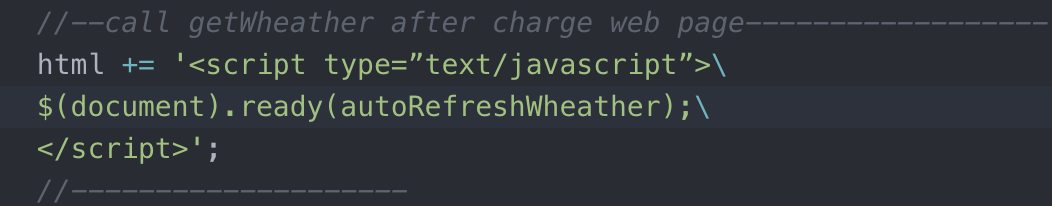
\includegraphics[width=0.8\textwidth]{callAutoRefresh.png}\\
				\caption cf.Données Json
			\end{minipage}%
		}%
\end{figure1}

La fonction \textbf{autoRefreshWheather} appelle la fonction \textbf{getWheather} toutes les 5 minutes.\\

\begin{figure1}
		\subfigure{
			\begin{minipage}[t]{\linewidth}
				\centering
				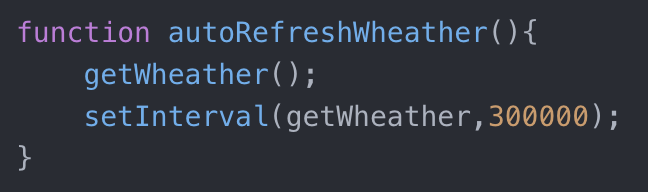
\includegraphics[width=0.8\textwidth]{reFresh.png}\\
				\caption cf.reFresh
			\end{minipage}%
		}%
\end{figure1}

La fonction \textbf{getWheather} envoie les informations correspondant à la ville du client au serveur et attend que le serveur renvoie les données json, puis affiche les données json sur html en appelant htmlWheather.

\begin{figure1}
		\subfigure{
			\begin{minipage}[t]{\linewidth}
				\centering
				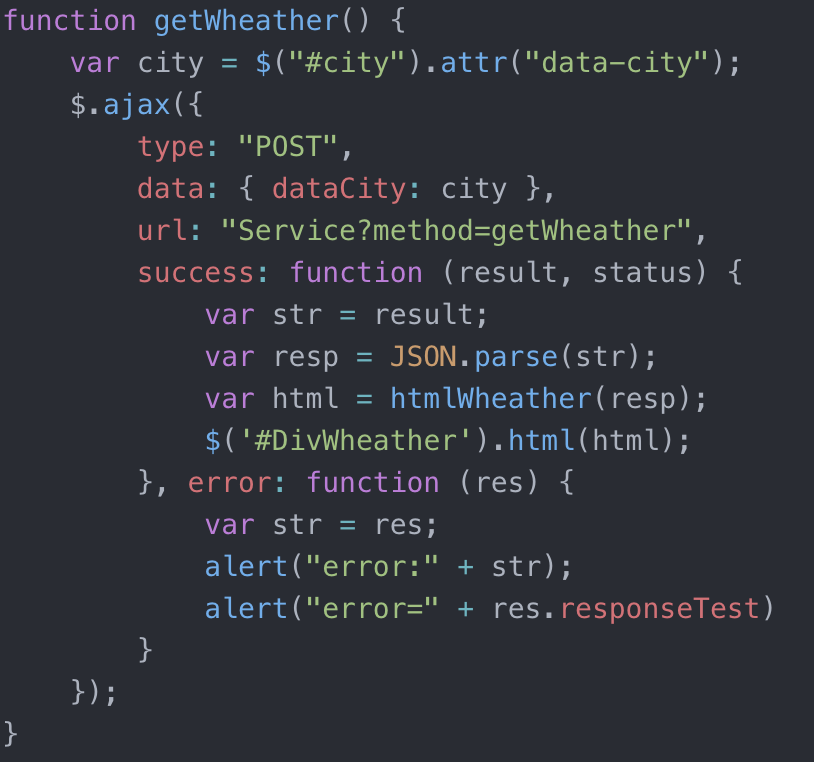
\includegraphics[width=0.8\textwidth]{getWheather.png}\\
				\caption cf.getWheather
			\end{minipage}%
		}%
\end{figure1}

Après réception de la demande, le serveur établit une connexion avec le serveur Weatherstack. Le serveur Weatherstack jugera s'il faut accepter la demande en fonction de la clé d'accès et retournera les données json en fonction de la valeur de la requête après avoir accepté la demande. Le serveur renvoie ensuite les données json au client via la méthode resp.getWriter().Write.\\

\begin{figure1}
		\subfigure{
			\begin{minipage}[t]{\linewidth}
				\centering
				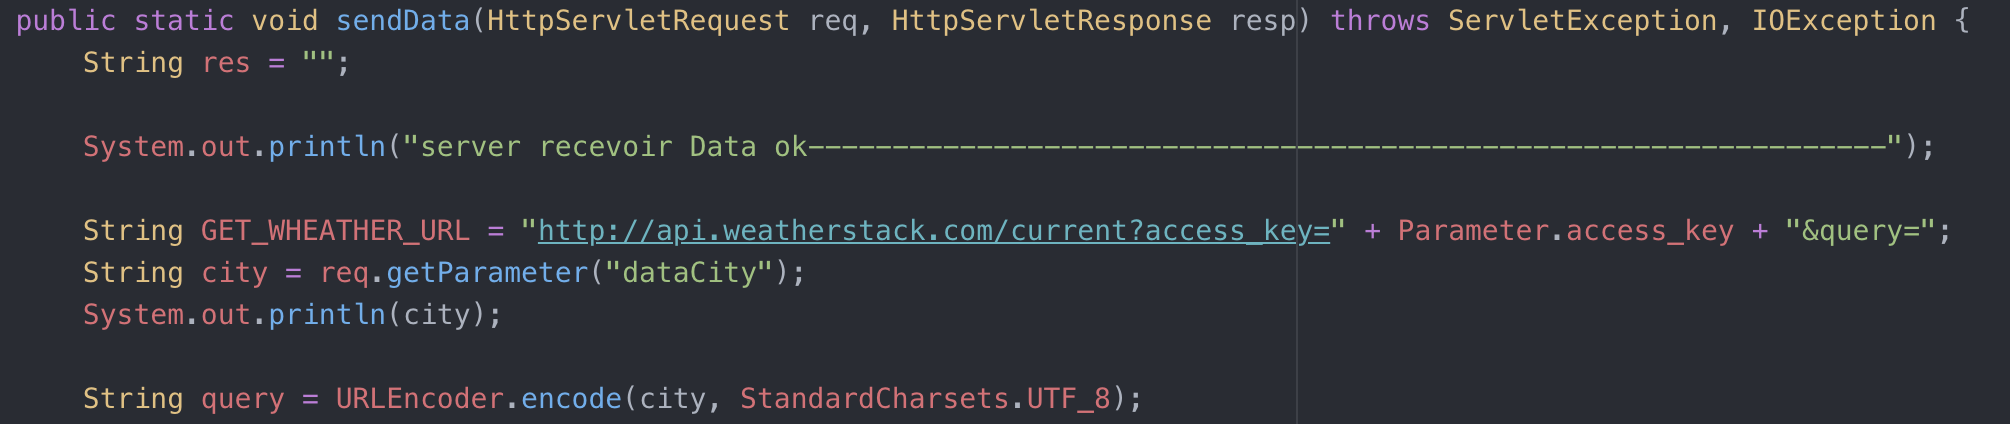
\includegraphics[width=1\textwidth]{setupConnection.png}\\
				\caption cf.setupConnection
			\end{minipage}%
		}%
\end{figure1}

Enfin, nous afficherons les résultats des données json sur html.

\begin{figure1}
		\subfigure{
			\begin{minipage}[t]{\linewidth}
				\centering
				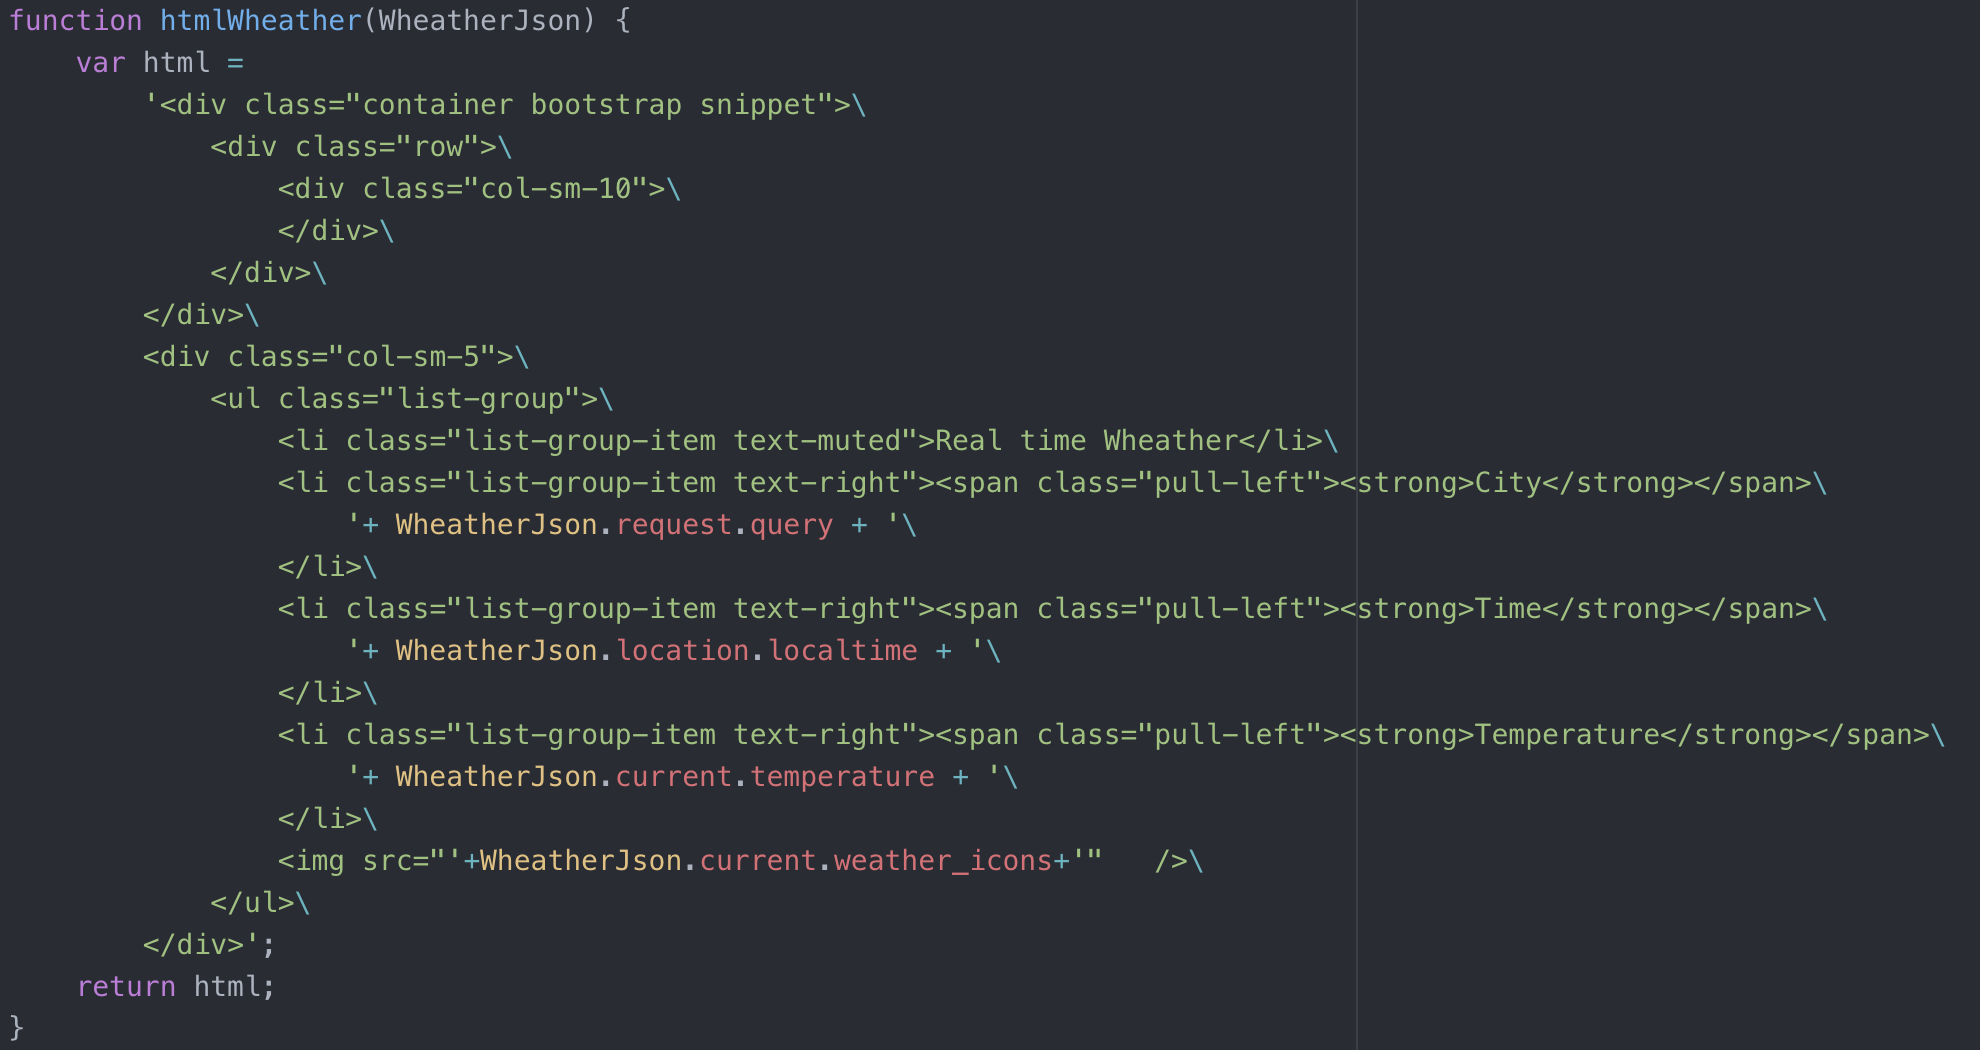
\includegraphics[width=1\textwidth]{htmlWheather.png}\\
				\caption cf.htmlWheather
			\end{minipage}%
		}%
\end{figure1}

\subsection{Mettre à jour Google Map}
Chaque fois ,l'utilisateur entre dans une page de détail de la propriété immobilière,	nous appellerons Google Maps pour localiser
la propriété immobilière.Le lien ci-dessous \textbf{googleapis} appellera en façon callback la méthode de js :\textbf{initMap}.
Il est à noter que le mot-clé \textbf{asyns} peut réaliser un chargement asynchrone, ce qui signifie que ce lien sera appelé après le chargement du HTML

\begin{figure1}
		\subfigure{
			\begin{minipage}[t]{\linewidth}
				\centering
				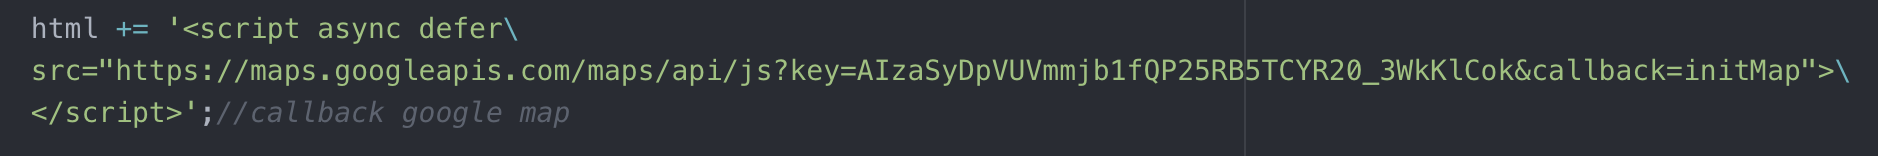
\includegraphics[width=1\textwidth]{htmlGoogleMaps.png}\\
				\caption cf.htmlWheather
			\end{minipage}%
		}%
\end{figure1}

Les fonctions initMap et geocodeAddress permettent à Google Maps de s'initialiser en fonction du lieu donné.

\begin{figure1}
		\subfigure{
			\begin{minipage}[t]{\linewidth}
				\centering
				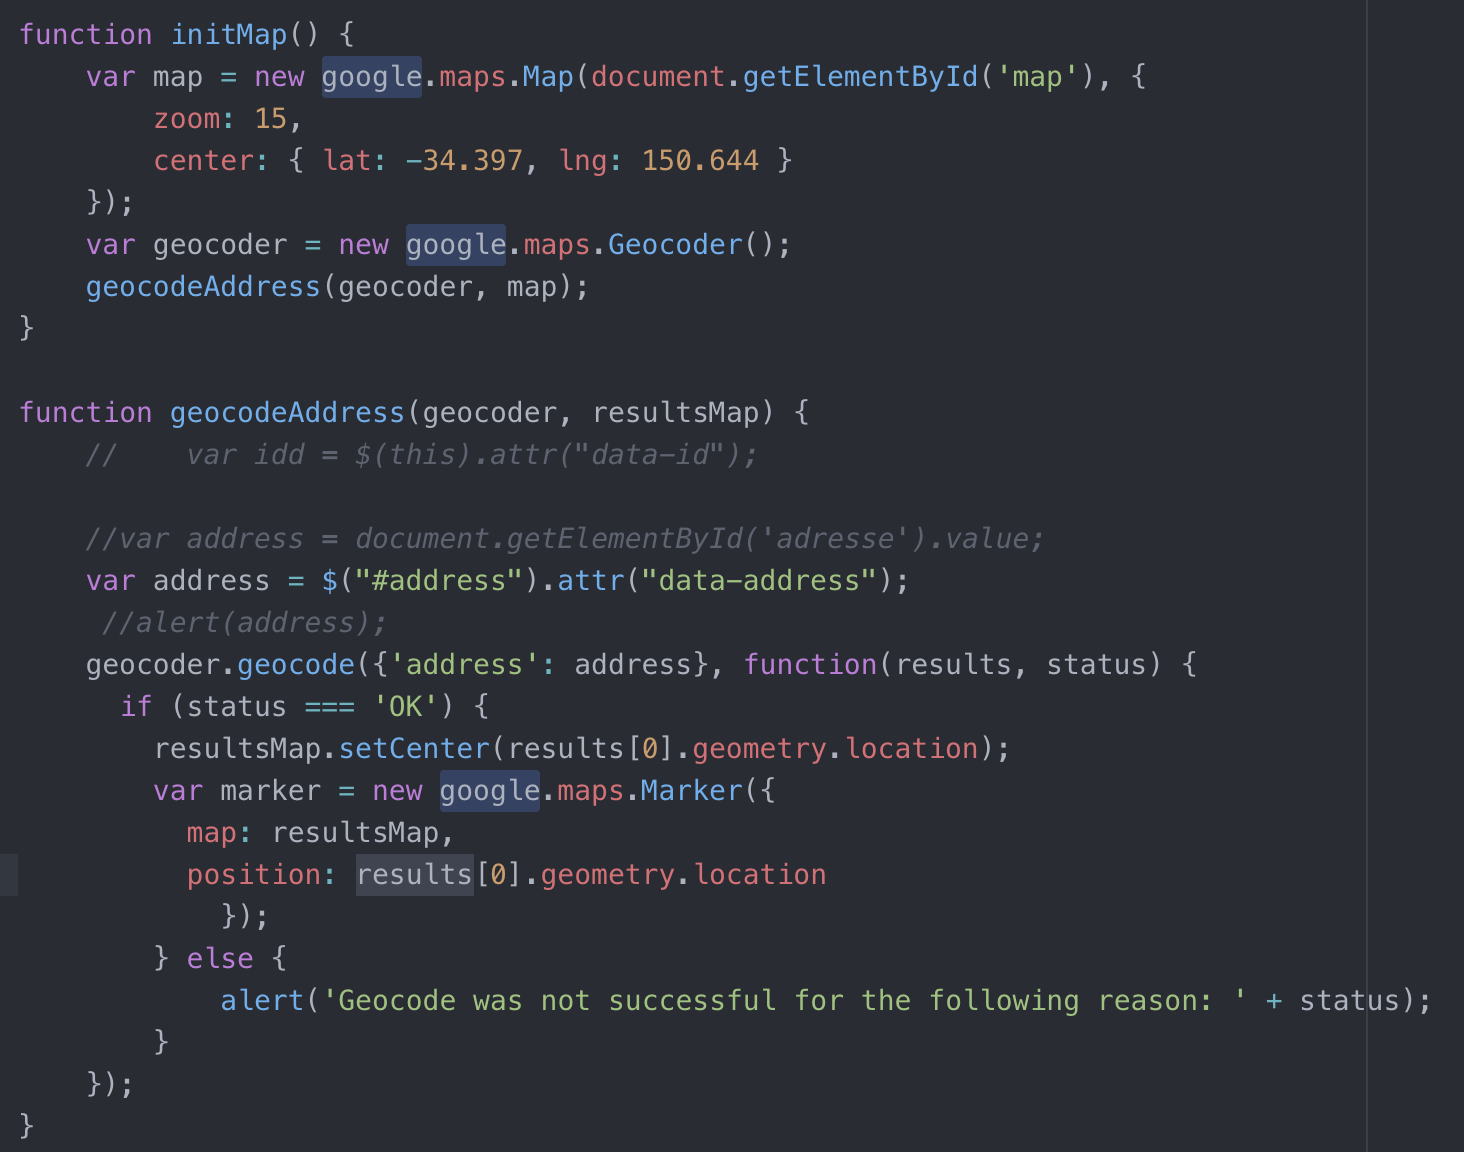
\includegraphics[width=1\textwidth]{initMaps.png}\\
				\caption cf.initMaps
			\end{minipage}%
		}%
\end{figure1}


\section{Fonctionnalités}
Le système est séparer en trois modules, \textbf{Account}, \textbf{Demand}, \textbf{Resource}. \\
Le module \textbf{Account} sert à gérer les données de l'authentification et l'espace de l'utilisateur. Le module \textbf{Resource} permet de gérer les données des logements. Et le module \textbf{Demand} sert à gérer les données des demands.\\
Cela permet de faciliter le développement parallèle et la maintenance de l'application. On a réaliser les fonctionnalités de l'ajoute, de la suppression et de la consultation, ainsi que la modification de ces trois modules.


\section{Cas d'utilisations}
\subsection{Module Compte}
\subsubsection{Inscription}
Acteur : L'utilisateur\\
Contexte : L'utilisateur crée un compte.\\
Scénario principal:
\begin{enumerate}
	\item L'utilisateur entre dans le page d'inscription.
	\item L'utilisateur saisit l'identifiant et le mot de passe.
	\item L'utilisateur clique Signup pour soumettre les information au serveur.
	\item Le système répond le message de success et afficher sur l'écran.
\end{enumerate}
Cas particulier:\\
4a. L'identifiant est déjà utilisé dans le système, le système affiche le message d'erreur.

\subsubsection{Authentification}
Acteur: L'utilisateur\\
Contexte: L'utilisateur s'authentifie dans le système par son compte.\\
Scénario principal:
\begin{enumerate}
	\item L'utilisateur entre dans le page de l'authentification.
	\item L'utilisateur saisit l'identifiant et le mot de passe.
	\item L'utilisateur clique le button \textbf{Login}.
	\item Le système vérifie l'identifiant et le mot de passe.
	\item Le système rend le page web de \textbf{mainPage.jsp}, l'identifiant est stocké dans la session.
\end{enumerate}
Cas particulier: \\
4a. L'identifiant n'est pas reconnu, le système affiche le message d'erreur.\\
4b. Le mot de passe n'est pas correspondant à l'identifiant, le système affiche le message d'erreur.

\subsubsection{Consulter l'espace du client}
Acteur: L'utilisateur\\
Contexte: L'utilisateur connecté veut consulter son espace du client.\\
Scénario principal:
\begin{enumerate}
	\item L'utilisateur clique le button Profile dans mainPage.
	\item Le système génère dynamiquement l'espace personnelle de l'utilisateur.
\end{enumerate}
cas particulier:\\
2a. L'utilisateur n'a pas encore son espace du client, le système génère le page de creation d'espace, permet à l'utilisateur de créer son espace.


\subsubsection{Créer l'espace du client}
Acteur: L'utilisateur\\
Contexte: L'utilisateur consulte sont espace première fois
Scénario principal:
\begin{enumerate}
	\item L'utilisateur clique le button Profile première fois dans le mainPage.
	\item Le système repond un message et génère dynamiquement le formulaire pour créer l'espace du client.
	\item L'utilisateur saisit les informations publiques.
	\item L'utilisateur clique le button \textbf{Créer}.
	\item Le système crée l'espace du client et le stocke dans la base de données, ainsi que génère le page web de l'espace du client.
\end{enumerate}

\subsubsection{Modifier l'espace du client}
Acteur: L'utilisateur\\
Contexte: L'utilisateur connecté se trouve dans son espace du client.\\
Scénario principal:
\begin{enumerate}
	\item L'utilisateur clique le button \textbf{here}.
	\item Le système génère un formulaire permet au client de modifier son espace.
	\item Le système remplit le formulaire selon les informations actuelles de l'utilisateur.
	\item L'utilisateur modifie ce qu'il veut changer.
	\item L'utilisateur clique le button \textbf{Modify}.
	\item Le système met à jour les informations de l'utilisateur.
\end{enumerate}

\subsection{Module Ressource}
\subsubsection{Consulter les ressources}
Acteur: L'utilisateur\\
Contexte: L'utilisateur s'authentifié se trouve à mainPage, il veut savoir le détail du logement.
Scénario principal:
\begin{enumerate}
	\item L'utilisateur clique le button \textbf{Your houses}.
	\item Le serveur cherche dans la base de donnée et génère dynamiquement le page sert à afficher les informations du logement, du propriétaire.
\end{enumerate}

\subsubsection{Ajouter la ressource}
Acteur: L'utilisateur\\
Contexte: L'utilisateur connecté se trouve dans le page \textbf{Your House}.\\
Scénario principal:
\begin{enumerate}
	\item L'utilisateur clique le button \textbf{Add House}.
	\item La page est générée dynamiquement par js permet à l'utilisateur de saisir les informations du logement.
	\item L'utilisateur clique le button \textbf{Créer}.
	\item Le système vérifie que le status de l'authentification de l'utilisateur est connecté.
	\item Le système stocke les informations du logement et affiche un message de la réussite sur l'écran.
\end{enumerate}

\subsubsection{Modifier la ressource}
Acteur: L'utilisateur\\
Contexte: L'utilisateur connecté se trouve dans la page du logement, il veut modifier les informations du logement.\\
Scénario principal:
\begin{enumerate}
	\item L'utilisateur clique le button \textbf{here}.
	\item Le système génère le formulaire de modification du logement.
	\item Le système remplit automatiquement le formulaire par les informations actuelles du logement.
	\item L'utilisateur modifie où il veut changer.
	\item L'utilisateur clique le button \textbf{Modify}.
	\item Le système met à jours les informations du logement et Le système affiche un message de la réussite sur l'écran.
\end{enumerate}

\subsubsection{Supprimer la ressource}
Acteur: L'utilisateur\\
Contexte: L'utilisateur connecté se trouve dans mainPage, il veut supprimer quelque logement.\\
Scénario principal:
\begin{enumerate}
	\item L'utilisateur clique le button \textbf{Your houses}.
	\item Le système cherche toutes les propriétés de l'utilisateur et les affiche sur une page générée automatiquement.
	\item L'utilisateur clique le button \textbf{delete} qui est à la même ligne avec le logement qu'il veut supprimer.
	\item Le système supprime le logement dans la base de donnée et affiche le message de la réussite sur l'écran.
\end{enumerate}
Cas particulier:
4a. Le logement est attaché par les demandes acceptées, le système ne peut pas le supprimer et affiche le message d'erreur sur l'écran.

\subsection{Module Demande}
\subsubsection{Réserver des logements}
Acteur: L'utilisateur\\
Contexte: L'utilisateur connecté se trouve dans mainPage, il veut réserver un ou plusieurs logements.\\
Scénario principal:
\begin{enumerate}
	\item L'utilisateur saisit la ville où il veut faire un séjour, le type du logement, la période du séjour, le droit de fumer et le nombre des voyageurs.
	\item L'utilisateur clique le button \textbf{Go}.
	\item Le système cherche tous les logements qui peut satisfaire les besoins.
	\item Le système filtre les logements dont le propriétaire est l'utilisateur lui-même.
	\item Le système affiche les restes logements sur l'écran.
	\item L'utilisateur clique le button \textbf{reserve} qui est sur la même ligne avec le logement que l'utilisateur veut réserver.
\end{enumerate}

\subsubsection{Consulter des demandes envoyées}
Acteur: L'utilisateur\\
Contexte: L'utilisateur connecté se trouve dans mainPage, il veut consulter les demandes envoyées.\\
Scénario principal:
\begin{enumerate}
	\item L'utilisateur clique le button \textbf{Sended demands}.
	\item Le système cherche les demandes envoyées par l'utilisateur dans la base de donnée et affiche sur une page générée automatiquement.
\end{enumerate}

\subsubsection{Consulter des demandes reçues}
Acteur: L'utilisateur\\
Contexte: L'utilisateur connecté se trouve dans mainPage, il veut consulter les demandes reçues.\\
Scénario principal:
\begin{enumerate}
	\item L'utilisateur clique le button \textbf{Recieved demands}.
	\item Le système cherche les demandes dont le logement est à l'utilisateur, et les affiche sur une page générée automatiquement.
\end{enumerate}

\subsubsection{Supprime des demandes envoyées}
Acteur: L'utilisateur\\
Contexte: L'utilisateur connecté se trouve dans la page \textbf{Sended demands}, il veut supprimer quelque demande.\\
Scénario principal:
\begin{enumerate}
	\item L'utilisateur clique le button \textbf{delete} qui est sur la même ligne avec la demande envoyée qu'il veut supprimer.
	\item Le système supprime la demande dans la base de donnée et affiche le message de la réussite sur l'écran.
\end{enumerate}

\subsubsection{Supprime des demandes reçues}
Acteur: L'utilisateur\\
Contexte: L'utilisateur connecté se trouve dans la page \textbf{Recieved demands}, il veut supprimer quelque demande.\\
Scénario principal:
\begin{enumerate}
	\item L'utilisateur clique le button \textbf{delete} qui est sur la même ligne avec la demande reçue qu'il veut supprimer.
	\item Le système supprime la demande dans la base de donnée et affiche le message de la réussite sur l'écran.
\end{enumerate}

\subsubsection{Accepter la demande}
Acteur: L'utilisateur\\
Contexte: L'utilisateur connecté se trouve dans la page \textbf{Recieved demands}, il veut accepter quelque demande.\\
Scénario principal:
\begin{enumerate}
	\item L'utilisateur clique le button \textbf{accept} qui est sur la même ligne avec la demande reçue qu'il veut accepter.
	\item Le système change l'état de demande de \textbf{Pending} à \textbf{Accepted}.
	\item Le système actualise les demandes et affiche un message de la réussite sur l'écran.
\end{enumerate}
Cas particulier:
2a. La demande cause un conflit avec une autre demande, le système refuse de modifier la base de donnée et affiche un message d'erreur sur l'écran.


\section{Stockage des données}
Les données sont stockées dans la base de données SQL, avec 4 quatre tables, la structure de ces 4 tables est comme indiqué ci-dessous.\\
\begin{figure1}
		\subfigure{
			\begin{minipage}[t]{\linewidth}
				\centering
				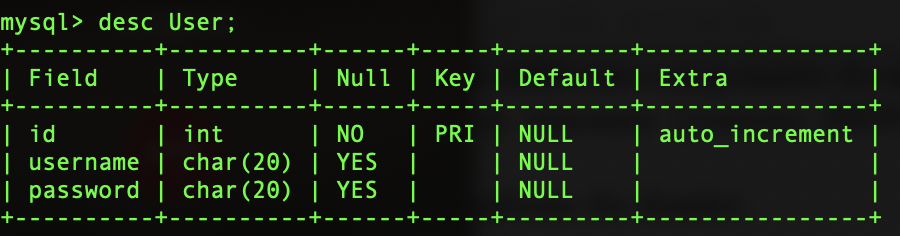
\includegraphics[width=0.5\textwidth]{tableUser.png}\\
				\caption cf.tableUser
			\end{minipage}%
		}%
\end{figure1}
\begin{figure1}
		\subfigure{
			\begin{minipage}[t]{\linewidth}
				\centering
				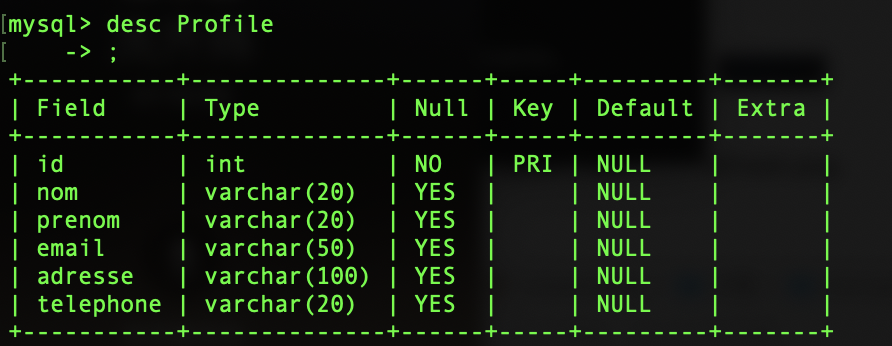
\includegraphics[width=0.5\textwidth]{tableProfile.png}\\
				\caption cf.tableProfile
			\end{minipage}%
		}%
\end{figure1}
\begin{figure1}
		\subfigure{
			\begin{minipage}[t]{\linewidth}
				\centering
				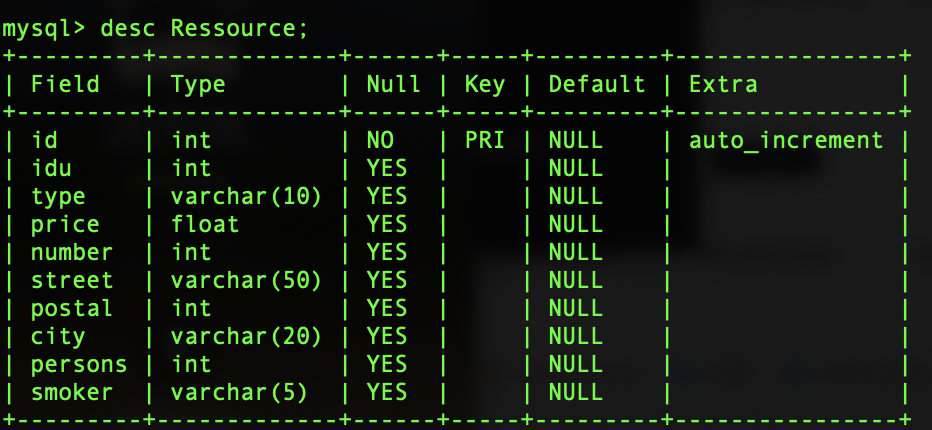
\includegraphics[width=0.5\textwidth]{tableRessource.png}\\
				\caption cf.tableRessource
			\end{minipage}%
		}%
\end{figure1}
\begin{figure1}
		\subfigure{
			\begin{minipage}[t]{\linewidth}
				\centering
				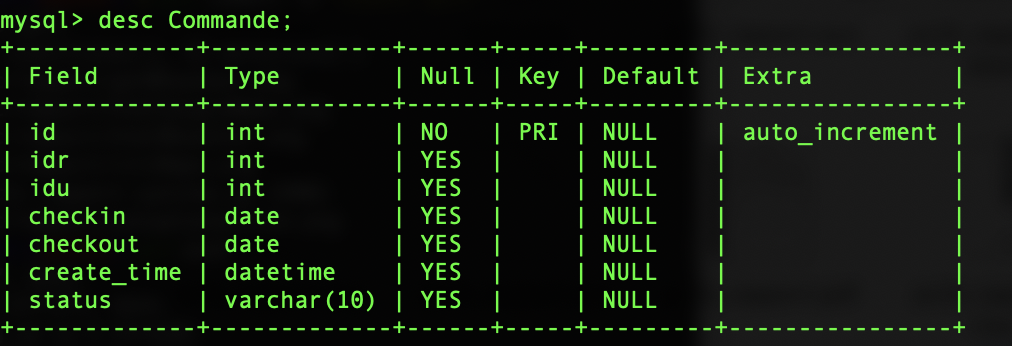
\includegraphics[width=0.5\textwidth]{tableCommande.png}\\
				\caption cf.tableCommande
			\end{minipage}%
		}%
\end{figure1}





\section{Structure du serveur}
La serveur se compose de quatres packages, \textbf{Bean}, \textbf{DAO}, \textbf{servlet} et \textbf{util}.

\subsection{Package Servlet}
Ce package possède les classes qui contient les \textbf{bisiness logic functions}.
Lors que l'utilisateur produit un événement comme appuie sur le bouton. Le client demande asynchronement au serveur par un URL. La classe \textbf{Service} sert à vérifier la demande et appeler la fonction correspondante.\\
Les fonctions pour gérer les informations du compte et s'authentification, ainsi que l'inscription sont réalisées dans \textbf{Client}\\
\textbf{Ressource} ont les méthodes servent à gérer les informations des logements.\\
\textbf{Gopage} permet de redirect à une autre page web.\\
\textbf{Demande} sert à gérer les information des demandes.\\
\textbf{Wheather} peut appeler API externe afin de rendre les informations du météo.

\subsection{Package Bean et DAO}
Dans la partie serveur, on utilise le pattern \textbf{DAO} afin d'encapsuler la manipulation de la base de donnée. \\
Le pattern \textbf{DAO} est l'abréviation de \textbf{Data Access Object}, pour chaque l'objet, on doit réaliser deux classes, \textbf{objetBean} et \textbf{objetDAO}.
\begin{enumerate}
	\item[-] Pour l'objetBean, il n'y a que les méthodes \textbf{get} et \textbf{set} et toutes les attributes sont privées, chaque attribute corresponde à chaque colonne de la table de base de donnée.
	\item[-] Pour l'objetDAO, il encapsule les manipulations, par exemple le stockage, la modification, la consultation et la suppression des données dans la base de données.
\end{enumerate}
Par conséquence on n'a pas besoin de répéter les instructions SQL, il ne suffit d'appeler les interfaces proposées par l'objetDAO. Ce parttern facilite de manipuler la base de donnnée et évite beaucoup d'erreur.

\subsection{Util}
Ce package a seulement deux classes, \textbf{Parameter} stocke des variables globales, par exemple l'identifiant et le mot de passe de base de données. \textbf{ToJson} est un objet pour créer une chaine de caractères en format de JSON.

\section{Structure du client}
\subsection{Le page jsp}
Cette application possède deux pages jsp, une est la page d'accueil. Après l'authentification de l'utilisation, l'utilisateur est redirect à la mainPage.jsp. Tous les contenus sont affichés sur cette page.
\subsection{JavaScript}
Nous avons séparer 7 fichiers \textbf{js} dans le projet.  
\begin{enumerate}
	\item \textbf{apiExterne.js} sert à l'appeler les APIs externes, GoogleMap et wheatherStack.
	\item \textbf{client.js} gère les événements du module \textbf{Account}. Par exemple, envoyer la requête au serveur pour créer et modifier l'espace de l'utilisateur.
	\item \textbf{demande.js} contient les fonctions concernant du module \textbf{Demande}. Par exemple, réserver un logement, accepter et supprimer la demande.
	\item \textbf{Ressource.js} sert à envoyer la requête concernant du module \textbf{Resource}, comme la consulation, la modification et la creation d'un logement.
	\item \textbf{htmlGenerator.js} permet de générer dynamiquement les contenus par un Json.
	\item \textbf{page.js} contrôle les effets de visualisation de page.
	\item \textbf{mainPage.js} attache tous les fonctions aux boutons.
\end{enumerate}



\section{Requêtes et réponse}
On utilise mainPage.js pour attacher les fonctions sur les boutons. Lors que les boutons sont appuyés, la fonction correspondante envoie asynchronement une requête aux client, la requête est un URL "Service?methode=xxxx\&parametre". Lors que le serveur reçoit ce URL, la classe \textbf{Service} peut savoir quelle fonction le client veut appeler. En plus, après l'exécution de la fonction correspondante, le serveur rend un json au client. Dès que le client reçoit le json, il va générer dynamiquement le contenu par la fonction de \textbf{htmlGenerator.js}.


\section{Annexe}
\begin{figure1}
		\subfigure{
			\begin{minipage}[t]{\linewidth}
				\centering
				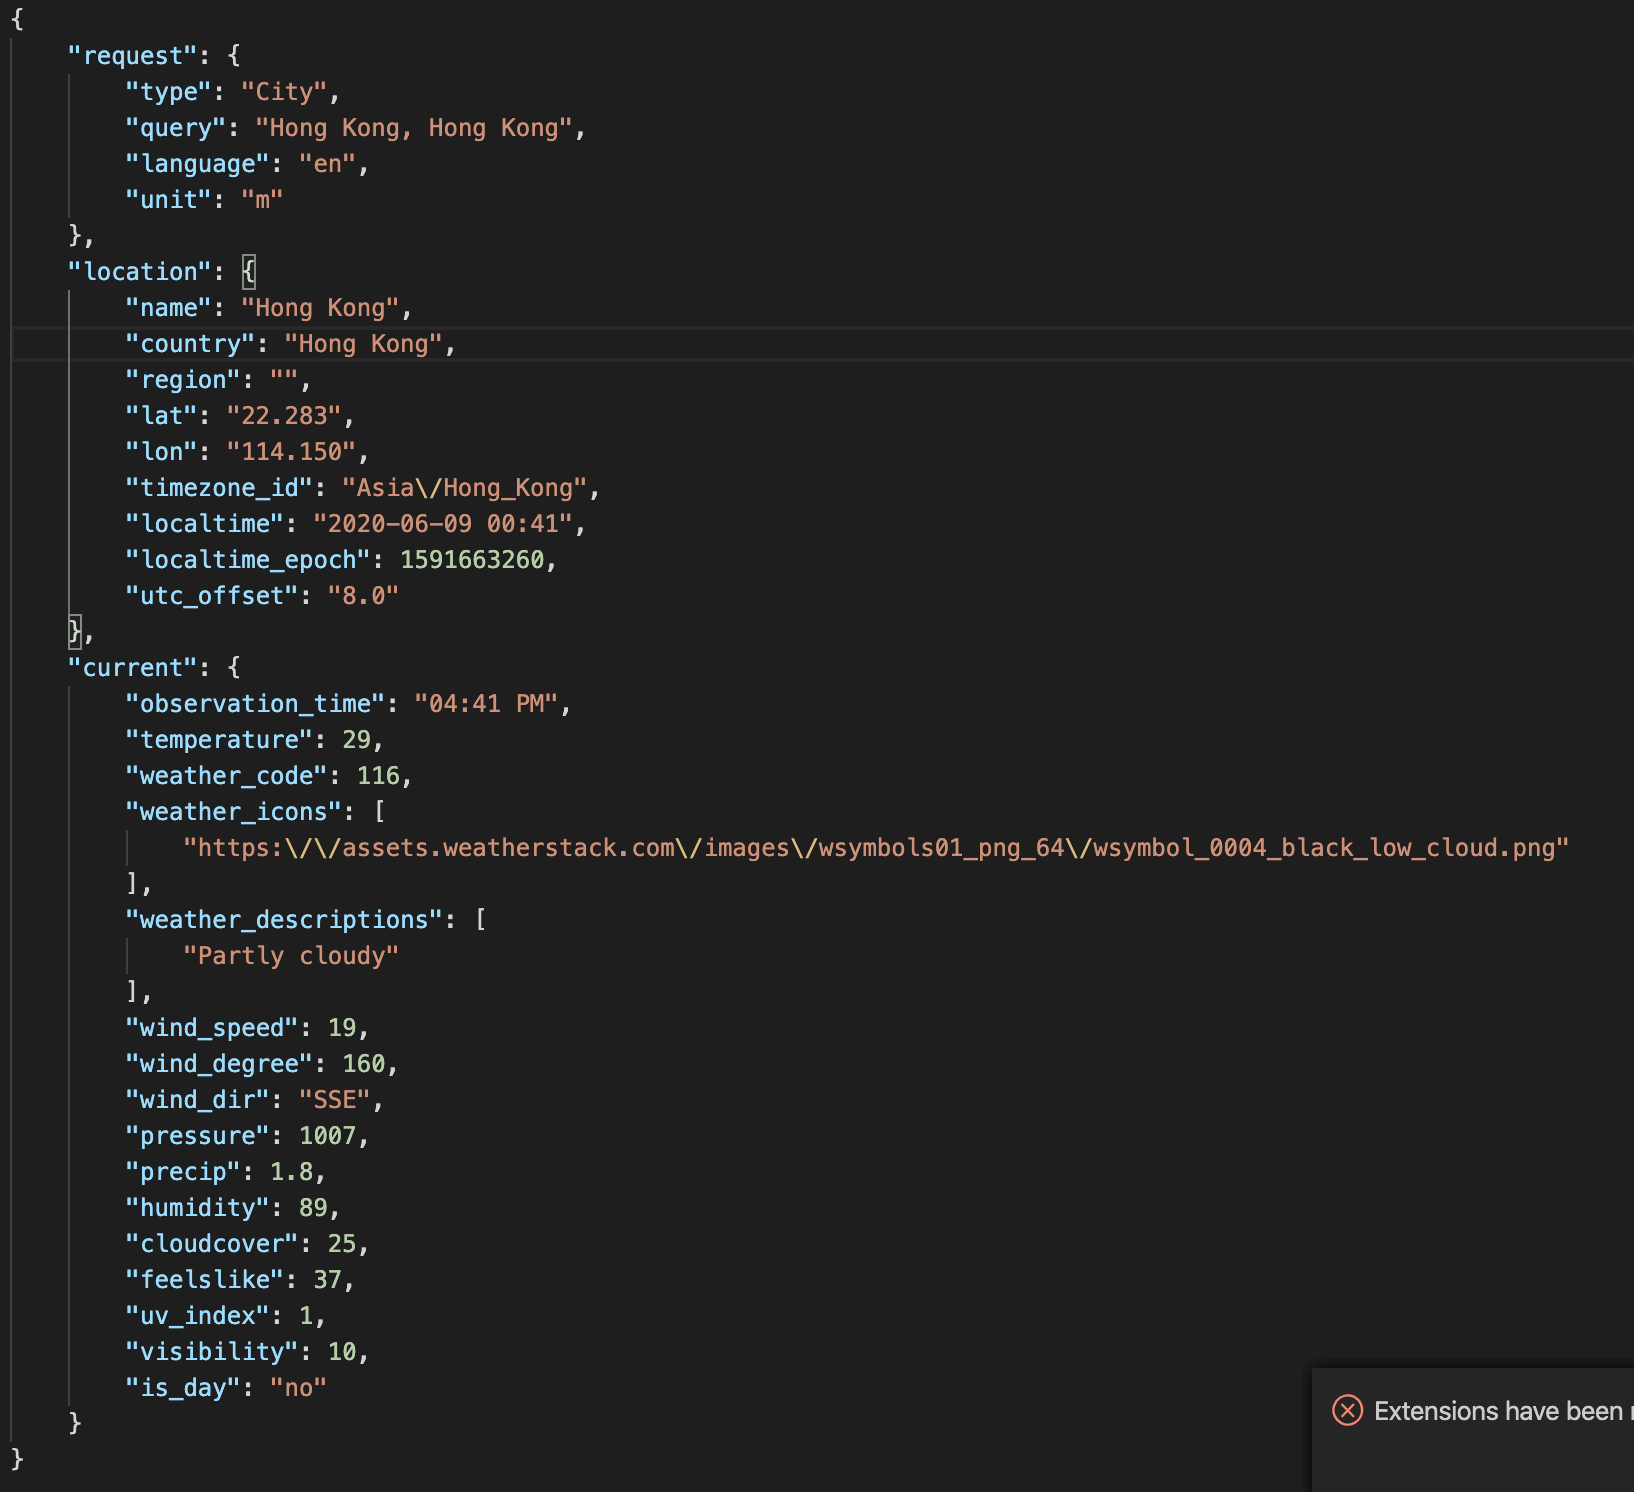
\includegraphics[width=0.8\textwidth]{json.png}\\
				\caption cf.Données Json
			\end{minipage}%
		}%
\end{figure1}

\begin{figure1}
		\subfigure{
			\begin{minipage}[t]{\linewidth}
				\centering
				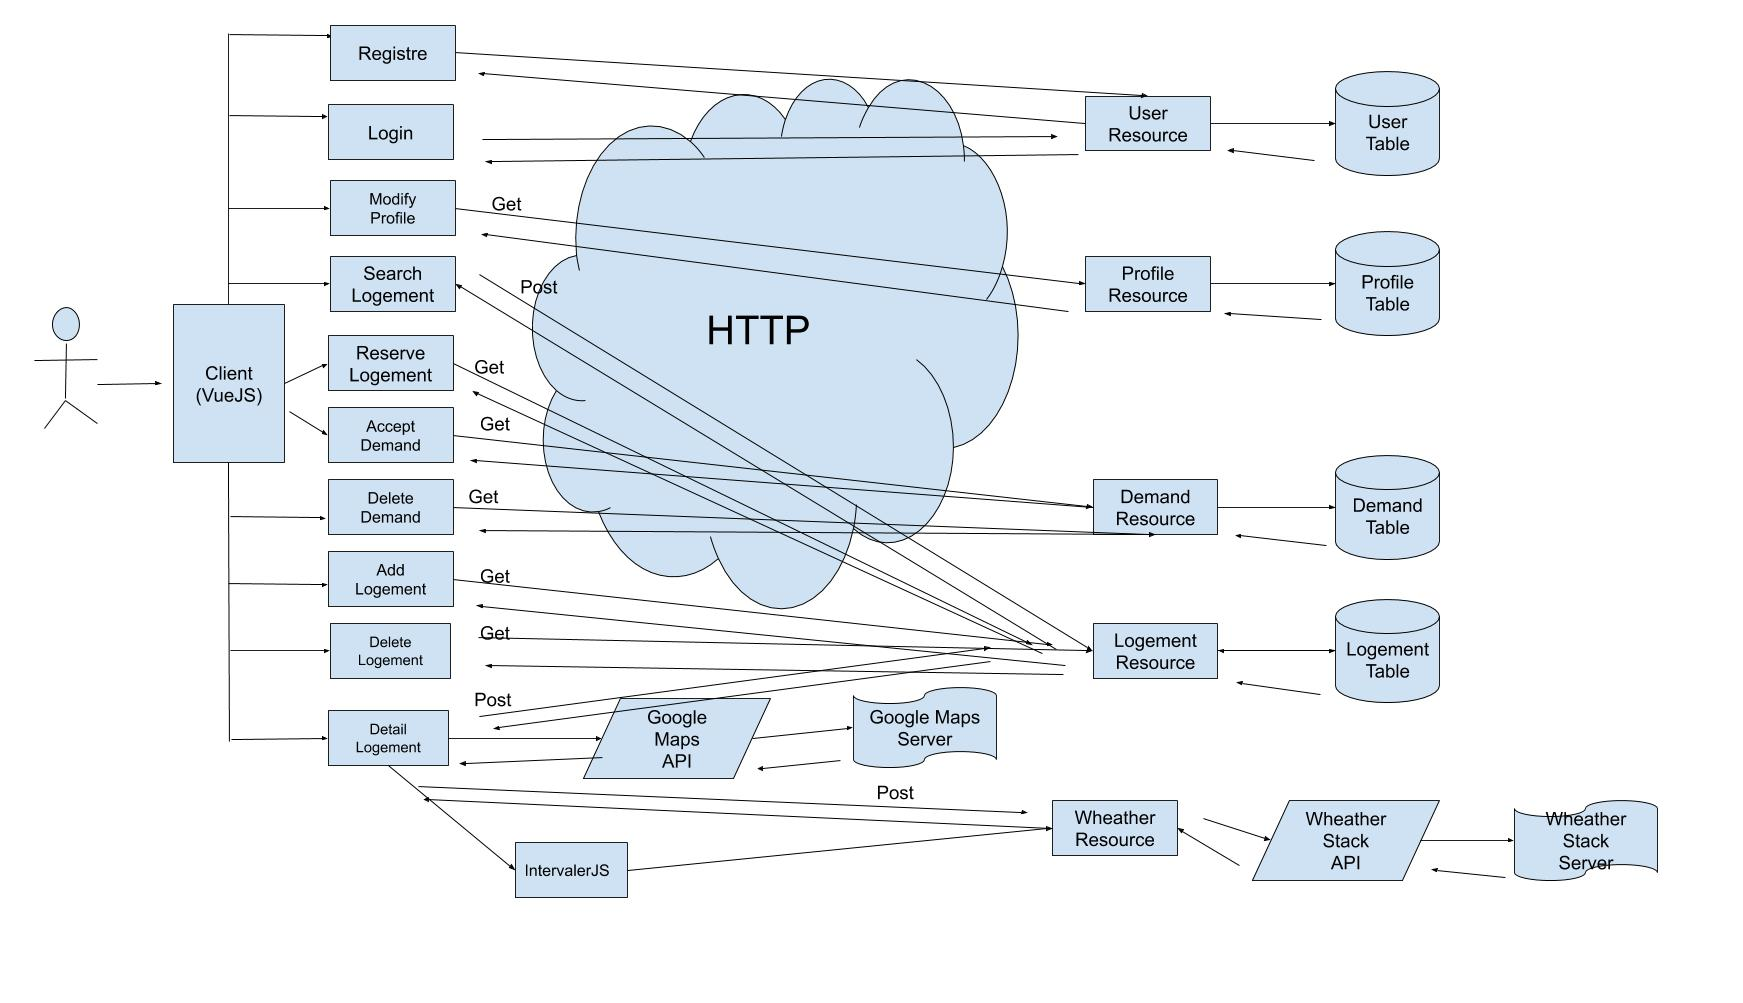
\includegraphics[width=0.8\textwidth]{schemaGlobal.jpg}\\
				\caption cf.Schéma global du système
			\end{minipage}%
		}%
\end{figure1}
\section{Référence}
[1]Weatherstack,[Online].Available:https://weatherstack.com/\\

[2]Google Maps,[Onlone].Available:https://cloud.google.com/maps-platform/\\



\end{document}
